\chapter{Prototipo}\label{ch:prototipo}
Questo capitolo descrive il progetto di prova finale realizzato durante il tirocinio, presso Gruppo SIGLA. In particolare, vengono discussi i tre livelli di sviluppo di un'applicazione web (il database, il back-end e il front-end) e le scelte progettuali fatte per realizzare il prototipo.

La parte di autenticazione all'applicazione web è stata gestita da Gruppo SIGLA tramite un sistema di autenticazione di terze parti, in modo da poter gestire gli accessi e le autorizzazioni degli utenti in modo centralizzato, usando i loro server esterni. Con questa decisione, il progetto non ha avuto la necessità di sviluppare login e registrazione degli utenti, ma si è concentrato sulle funzionalità di tracciamento e feedback delle attività formative erogate dall'azienda.

\begin{figure}[H]
\centering
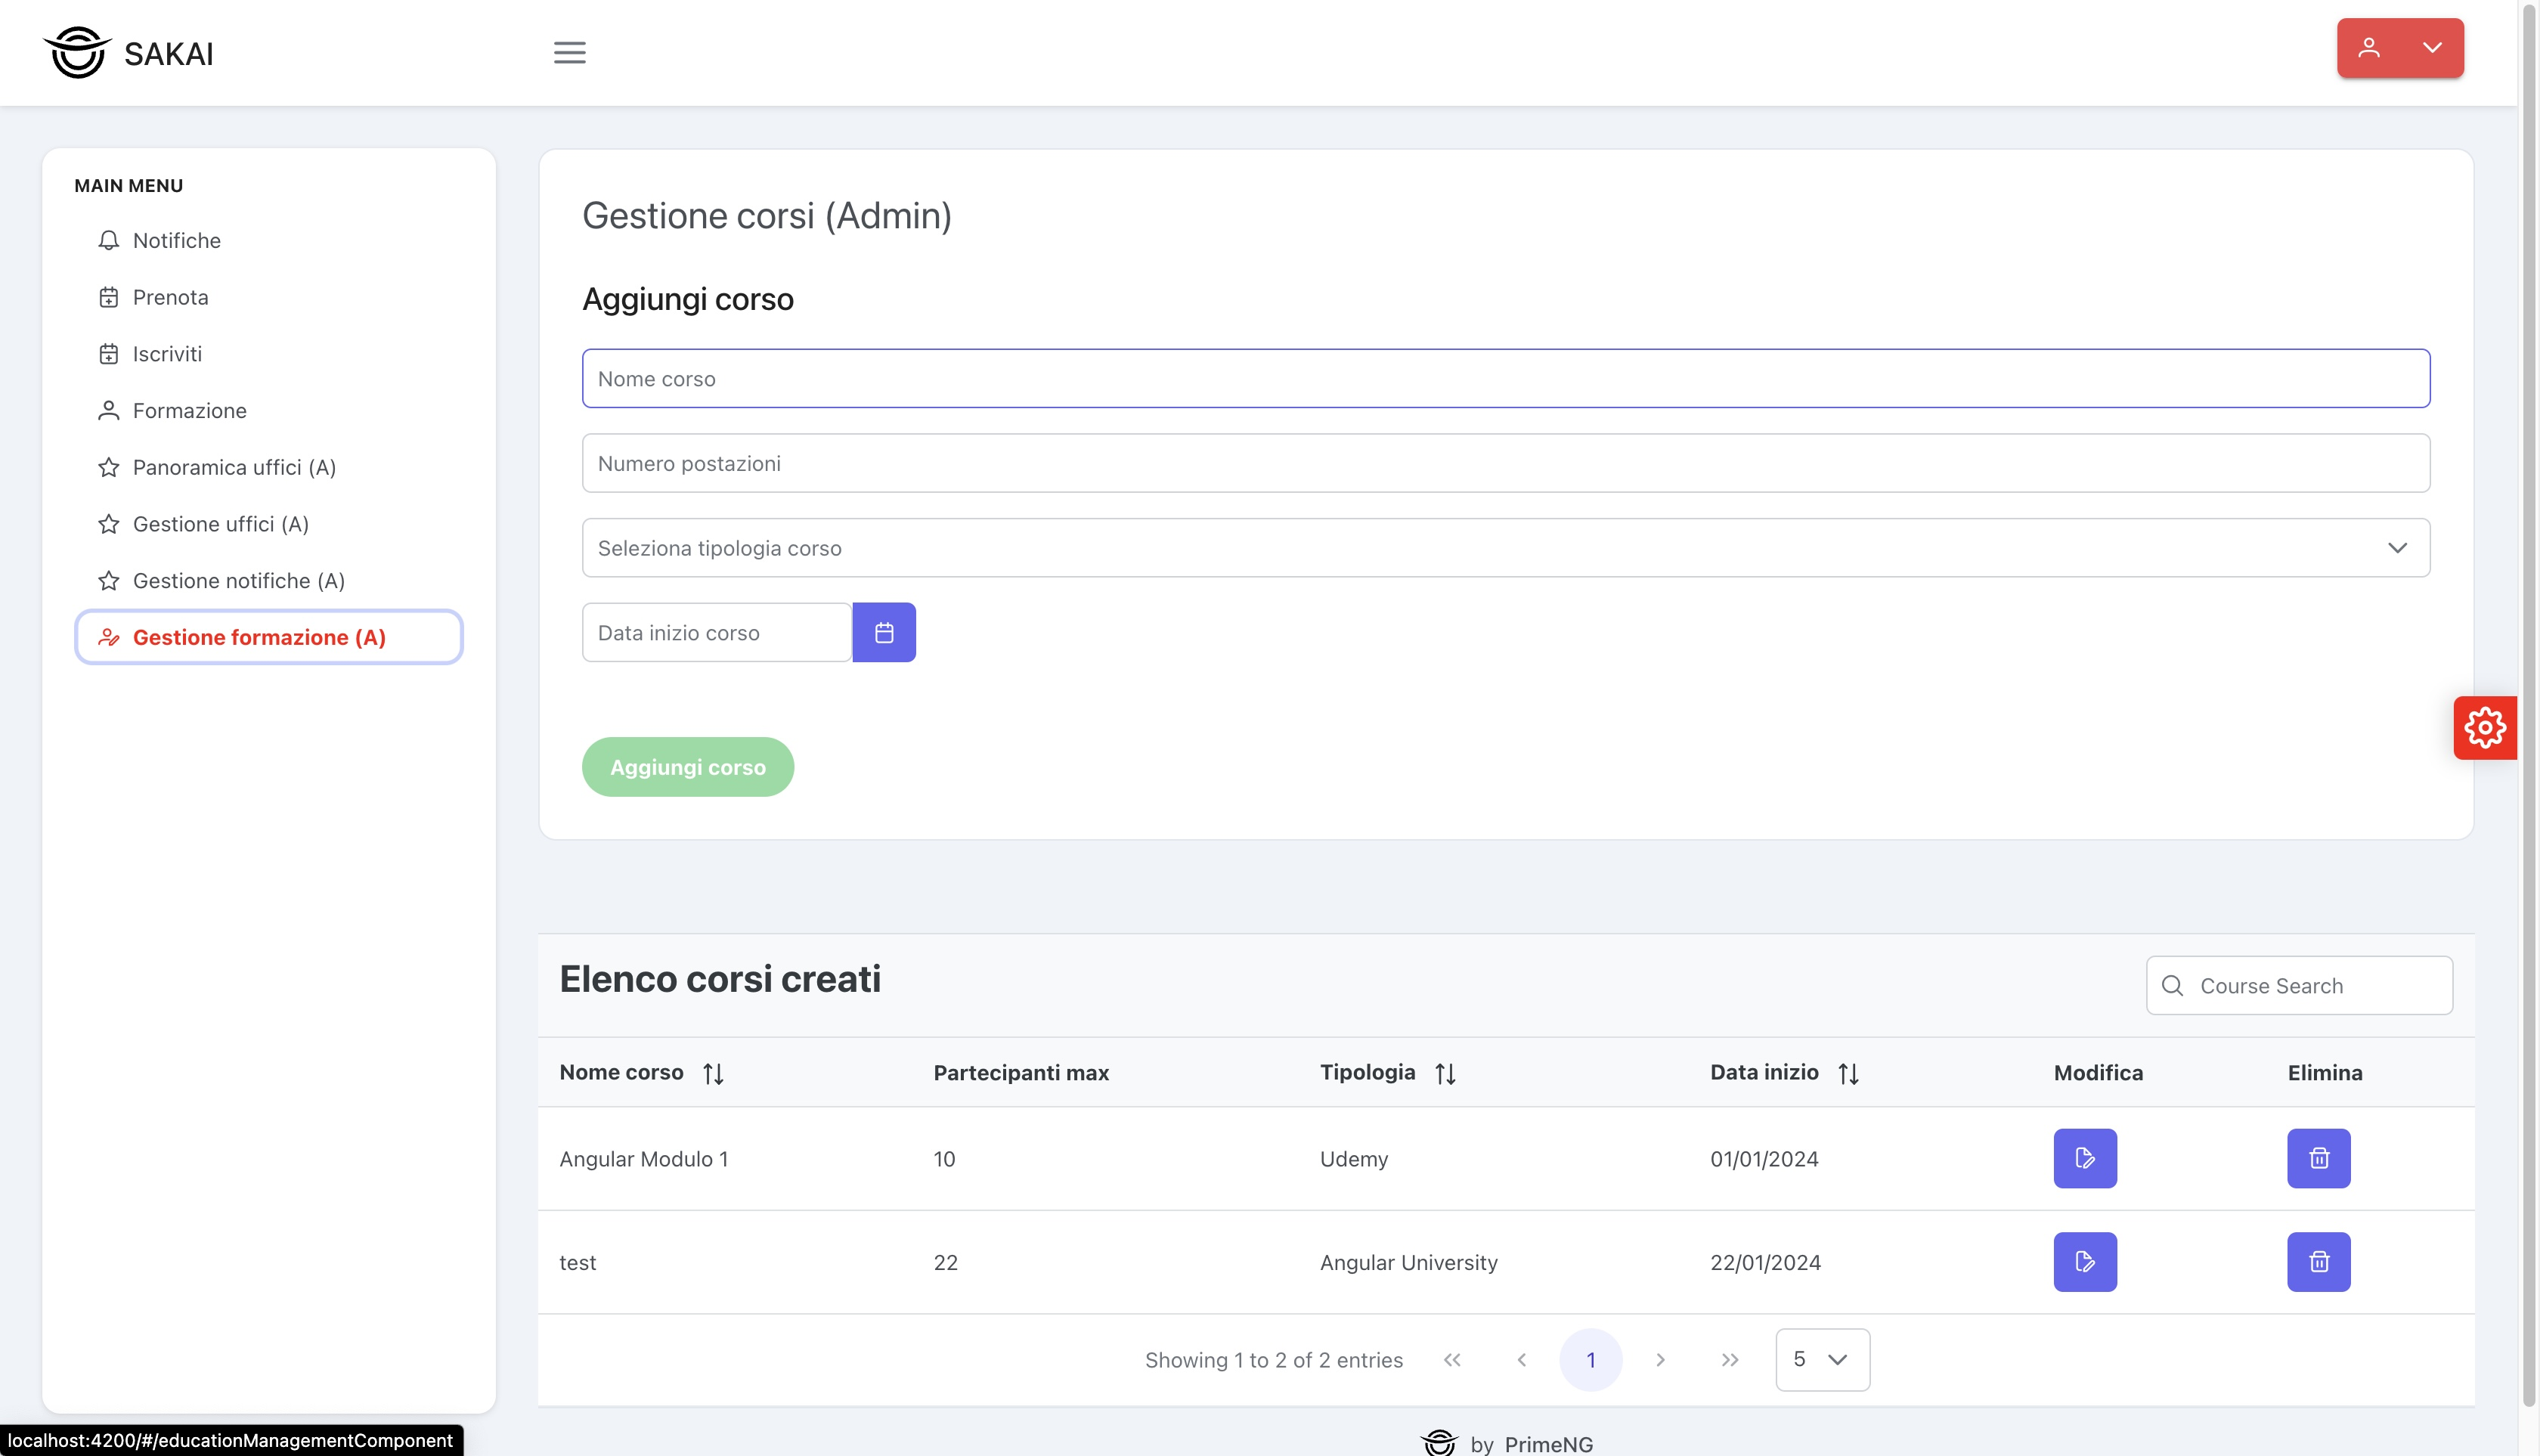
\includegraphics[width=1\textwidth]{Images/portale.jpg}
\caption{\label{fig:portale}Prototipo finale.}
\end{figure}

La figura \ref{fig:portale} mostra una delle pagine del prototipo.

% DB %%%%%%%%%%%%%%%%%%%%%%%%%%%%%%%%%%%%%%%%%%%%%%%%%%%%%%%%%%%%%%%%%%%%%%%%%%%%%%%%%%%%%%%%%%%%%%%%%%%%%%%%
\section{Database}\label{sec:database}
Innanzitutto è stato necessario progettare il database, nello specifico, la creazione di tabelle contenenti le tuple di prova per effettuare il test del prototipo. 
Come da richiesta di Gruppo SIGLA, non è stata realizzata la tabella per la gestione degli utenti, in quanto il progetto di tirocinio si è concentrato principalmente sulle funzionalità dell'amministratore per aggiungere, modificare ed eliminare le attività formative, erogate dall'azienda.

Grazie alle \acrshort{api} di \acrshort{asp.net}, è stato possibile creare la tabella del database direttamente dal codice del back-end. Quindi, è stato utilizzato un \acrfull{orm}, una tecnica che si usa per convertire i dati tra un database relazionale e lo heap\footnote{\glsdesc{heap}} di un linguaggio di programmazione orientato agli oggetti \cite{articleORM}.

Per la tabella dei corsi di formazione, sono stati creati i seguenti campi: 
\begin{itemize}
  \item \texttt{Id del corso} (integer), chiave primaria
  \item \texttt{CoursesName} (string), nome del corso
  \item \texttt{CoursesCapacity} (integer), capacità massima di utenti del corso
  \item \texttt{CoursesType} (string), tipologia del corso
  \item \texttt{CoursesDate} (string), data di inizio del corso
\end{itemize}

Una volta fatto ciò, la tabella che tiene traccia delle versioni del database, `VersionInfo' è stata aggiornata con le nuove migrazioni\footnote{\glsdesc{migrazione}}. Le sue colonne sono:
\begin{itemize}
  \item \texttt{Version} (integer), versione del database
  \item \texttt{AppliedOn} (datetime), data di applicazione della migrazione
  \item \texttt{Description} (text), descrizione della migrazione
\end{itemize}

Per visualizzare e gestire il database, è stato utilizzato DBeaver, un software gratuito e open source per la gestione di database relazionali. La scelta di usare DBeaver è dovuta alla sua semplicità d'uso e al fatto che sia sviluppato dalla comunità open source \cite{dbeaver}.

\begin{figure}[H]
\centering

\includegraphics[width=0.25\textwidth]{Images/dbeaver.png}
\caption{\label{fig:dbeaver}Logo di DBeaver.}
\end{figure}


% back-end %%%%%%%%%%%%%%%%%%%%%%%%%%%%%%%%%%%%%%%%%%%%%%%%%%%%%%%%%%%%%%%%%%%%%%%%%%%%%%%%%%%%%%%%%%%%%%%%%%%%
 
\section{Back-end}\label{sec:back-end}
Questa sezione descrive come ho usato \acrshort{asp.net} per lo sviluppo del back-end del prototipo.

Lo sviluppo principale è stato fatto appoggiandosi all'applicazione web già esistente, sulla quale Gruppo SIGLA ha sviluppato il progetto di tirocinio, che poi offre agli studenti. Quindi, basandomi sull'architettura già esistente, ho creato 5 nuove classi e modificato la classe \texttt{Program.cs}, già esistente, per gestire le funzionalità del prototipo. Queste classi sono:
\begin{itemize}
  \item \texttt{CoursesData.cs}
  \item \texttt{4\_CoursesMigration.cs}
  \item \texttt{CoursesController.cs}
  \item \texttt{CoursesDataGetListExecutor.cs}
  \item \texttt{CoursesDataExecuteExecutor.cs}
\end{itemize}

In particolare, la classe \texttt{CoursesData.cs} è stata creata per definire la tabella `CoursesData' e le sue colonne, tramite la libreria IdentityModel di \acrshort{asp.net}. La classe viene gestita come un'entità grazie all'attributo \texttt{[DbModel]} e le colonne vengono definite come proprietà della classe stessa, coi rispettivi metodi getter\footnote{\glsdesc{getter}} e setter\footnote{\glsdesc{setter}}.
La figura \ref{fig:coursesdata} mostra il codice C\# del file \texttt{CoursesData.cs}.

\begin{figure}[H]
\begin{lstlisting}[linewidth=20cm, captionpos=b]
namespace It.gs.back-end.Model
{
  using System.Text.Json.Serialization;
  using It.gs.Repository;
  using It.gs.Repository.Model;
  public class AddCoursesToDbExecuteInfo : IExecuteInfo {
    public CoursesData[] Courses {get; set; }
  }
  public class DeleteCoursesDataExecuteInfo : IExecuteInfo {
    public CoursesData[] Courses {get; set; }
  }
  public class UpdateCoursesDataExecuteInfo : IExecuteInfo {
    public CoursesData[] Courses {get; set; }
  }
  [DbModel]
  public class CoursesData
  {
      [JsonPropertyName("coursesId")]
      public int CoursesId { get; set; }
    
      [JsonPropertyName("coursesName")]
      public string CoursesName { get; set; }
    
      [JsonPropertyName("coursesCapacity")]
      public int CoursesCapacity { get; set; }
    
      [JsonPropertyName("coursesType")]
      public string CoursesType { get; set; }
    
      [JsonPropertyName("coursesDate")]
      public string CoursesDate { get; set; }
    
      [JsonPropertyName("count")]
      public int? Count { get; set; }
  }
}
\end{lstlisting}
\caption{\label{fig:coursesdata}Codice in C\# del file \texttt{CoursesData.cs}.}
\end{figure}

La classe \texttt{CoursesMigration}, che estende la classe del contesto \texttt{Migration}, si occupa di creare la tabella del database, tramite un \acrshort{orm} \cite{orm} e i metodi appositi della libreria \texttt{FluentMigrator} \cite{fluentmigrator}. In figura \ref{fig:coursesdata} si può vedere il listato del codice relativo alla creazione del database.
\begin{figure}[H]
\begin{lstlisting}
Create.Table($"{nameof(CoursesData)}")
    .WithColumn($"{nameof(CoursesData.CoursesId)}") .AsInt32() .PrimaryKey().Identity()
    .WithColumn($"{nameof(CoursesData.CoursesName)}") .AsBoolean() .NotNullable().WithDefaultValue(false)
    .WithColumn($"{nameof(CoursesData.CoursesCapacity)}") .AsInt16() .NotNullable().WithDefaultValue(10)
    .WithColumn($"{nameof(CoursesData.CoursesType)}") .AsString() .NotNullable()
    .WithColumn($"{nameof(CoursesData.CoursesDate)}") .AsString() .NotNullable();
\end{lstlisting}
\caption{\label{fig:migration}Frammento di codice C\# del file \texttt{4\_CoursesMigration.cs}.}
\end{figure}
Il listato si trova all'interno del metodo \texttt{Up()} della classe \texttt{CoursesMigration}. 

Siccome i metodi \texttt{Up()} e \texttt{Down()} sono ereditati dalla libreria \texttt{FluentMigrator}, è necessario fare un override\footnote{\glsdesc{override}}, riscrivendoli.

Successivamente, ho inizializzato delle tuple di prova all'interno di una lista denominata \texttt{coursesRows} e le ho inserite nella tabella appena creata tramite un ciclo di scorrimento. In figura \ref{fig:insert} si può vedere il listato appena discusso.
\begin{figure}[H]
\begin{lstlisting}
foreach(var course in coursesRows)
    Insert.IntoTable($"{nameof(CoursesData)}").Row(course);
\end{lstlisting}
\caption{\label{fig:insert}Frammento di codice C\# del file \texttt{4\_CoursesMigration.cs}.}
\end{figure}

La classe \texttt{CoursesController}, invece, estende la classe \texttt{ControllerBase}. In particolare, grazie agli attributi \texttt{[HttpPost(" ")]} e \texttt{[ProducesResponseType(400)]}, gestisce le richieste e le risposte \acrshort{http}, smistandole nei metodi responsabili di ognuna delle operazioni (aggiunta, modifica, ricerca o eliminazione). Per esempio, il metodo \texttt{AddCoursesToDb} crea un oggetto contenente le informazioni necessarie all'esecuzione e lo passa come parametro al metodo \texttt{Execute} che eseguirà una delle quattro azioni, a seconda del tipo dell'oggetto in input. In figura \ref{fig:add} si può vedere il listato del metodo appena discusso.
\begin{figure}[H]
\begin{lstlisting}
[HttpPost("addCoursesData")]
[ProducesResponseType(200)]
[ProducesResponseType(400)]
[ProducesResponseType(500)]
public async Task<IActionResult> AddCoursesToDb([FromBody] CoursesData[] Courses) {
    var CoursesInfo = new AddCoursesToDbExecuteInfo {Courses = Courses};
    var result = await this.coursesDataRepo.Execute(CoursesInfo);
    if(result.IsSuccess)
        return Ok();
    else 
        throw result.Error.SourceException;
}
\end{lstlisting}
\caption{\label{fig:add}Metodo \texttt{AddCoursesToDb()} in C\#, del file \texttt{CoursesController.cs}.}
\end{figure}
I metodi relativi alle altre operazioni sono analoghi al codice in figura \ref{fig:add}.


Il metodo \texttt{Execute(...)} è all'interno della classe \texttt{CoursesDataExecuteExecutor}, che si occupa di eseguire l'operazione corretta, a seconda del tipo dell'oggetto (\texttt{info}) che riceve in input. In figura \ref{fig:switch} si può vedere il listato del codice che gestisce lo smistamento delle operazioni.
\begin{figure}[H]
\begin{lstlisting}
public async Task<IExecuteResult> Execute(DatabaseSettings settings, IDbConnection connection, IDbTransaction transaction, IExecuteInfo info)
{
    switch(info) {
        case AddCoursesToDbExecuteInfo i: 
            return await AddCoursesExecute(settings, connection, transaction, i);
        case DeleteCoursesDataExecuteInfo i:
            return await DeleteCoursesDataExecute(settings, connection, transaction, i);
        case UpdateCoursesDataExecuteInfo i:
            return await UpdateCoursesDataExecute(settings, connection, transaction, i);
        default:
            throw new NotSupportedException($"Execute with transaction for type {info.GetType().FullName} not supported");
    }
}
\end{lstlisting}
\caption{\label{fig:switch}Metodo C\# \texttt{Execute()} contenente lo \texttt{switch} relativo alle operazioni.}
\end{figure}

Nel caso in cui \texttt{info} sia di tipo \texttt{AddCoursesToDbExecuteInfo}, verranno eseguiti i metodi \texttt{AddCoursesExecute} e \texttt{Add}, relativi all'aggiunta di una riga alla tabella dei corsi, come si può vedere nei frammenti di codice delle figure \ref{fig:adding} e \ref{fig:get list}.

\begin{figure}[H]
\begin{lstlisting}
private async Task<IExecuteResult> AddCoursesExecute(DatabaseSettings settings, IDbConnection connection, IDbTransaction transaction, AddCoursesToDbExecuteInfo info) {
    foreach(var Course in info.Courses) {
        _ = await Add(settings, connection, transaction, Course);
    }

    return await IExecuteResult.From(\texttt{true});
}
private async Task<CoursesData> Add(DatabaseSettings settings, IDbConnection connection, IDbTransaction transaction, CoursesData item)
{
    Console.WriteLine("item: ",item);
    var sql = $"INSERT INTO CoursesData (CoursesName, CoursesCapacity, CoursesType, CoursesDate) VALUES (@{nameof(CoursesData.CoursesName)}, @{nameof(CoursesData.CoursesCapacity)}, @{nameof(CoursesData.CoursesType)}, @{nameof(CoursesData.CoursesDate)})";

    var r = await connection.ExecuteAsync(sql, item, transaction);
    return item;
}
\end{lstlisting}
\caption{\label{fig:adding}Metodi C\# per l'inserimento dei corsi nel database.}
\end{figure}
In particolare, notiamo che \texttt{AddCoursesToDbExecuteInfo()} chiama \texttt{Add()} e in quest'ultimo vengono effettivamente implementate le query per interrogare il database.

Infine, è degno di nota anche il file \texttt{CoursesDataGetListExecutor.cs}, che si occupa di raccogliere la lista dei corsi di formazione, tramite il metodo \texttt{GetList()}, chiamato dalla classe \texttt{CoursesController} descritta in precedenza.

\begin{figure}[H]
\centerline{(Listato \ref{fig:get list}).}
\begin{lstlisting}
public async Task<IEnumerable<CoursesData>> GetList(DatabaseSettings settings, IDbConnection connection, Maybe<CoreDynamicQueryPart> query)
{
    var (countSql, sql, parameters) = query.EnsureOrderBy(nameof(CoursesData.CoursesId)) .ComposeWithCount<DapperQueryParametersBuilder, DynamicParameters>($"SELECT * $FROM {nameof(CoursesData)}", nameof(CoursesData.CoursesId), settings);
    var result = await connection.QueryAsync<CoursesData>(sql: sql, param: parameters);
    var count = await connection.QuerySingleAsync<int>(sql: countSql, param: parameters);
    return result.Select(x => { x.Count = count; return x; });
}
\end{lstlisting}
\caption{\label{fig:get list}Implementazione del metodo \texttt{GetList.cs} del file C\#  \texttt{CoursesDataGetListExecutor.cs}.}
\end{figure}

Una volta implementato il back-end, per verificare il suo corretto funzionamento, ho utilizzato una \acrshort{api} apposita, Swagger, già discussa nel Capitolo \ref{ch:Contesto}. Nelle figure \ref{fig:swagger courses} e \ref{fig:swagger success} si possono vedere alcuni esempi di utilizzo.

\begin{figure}[H]
\centering
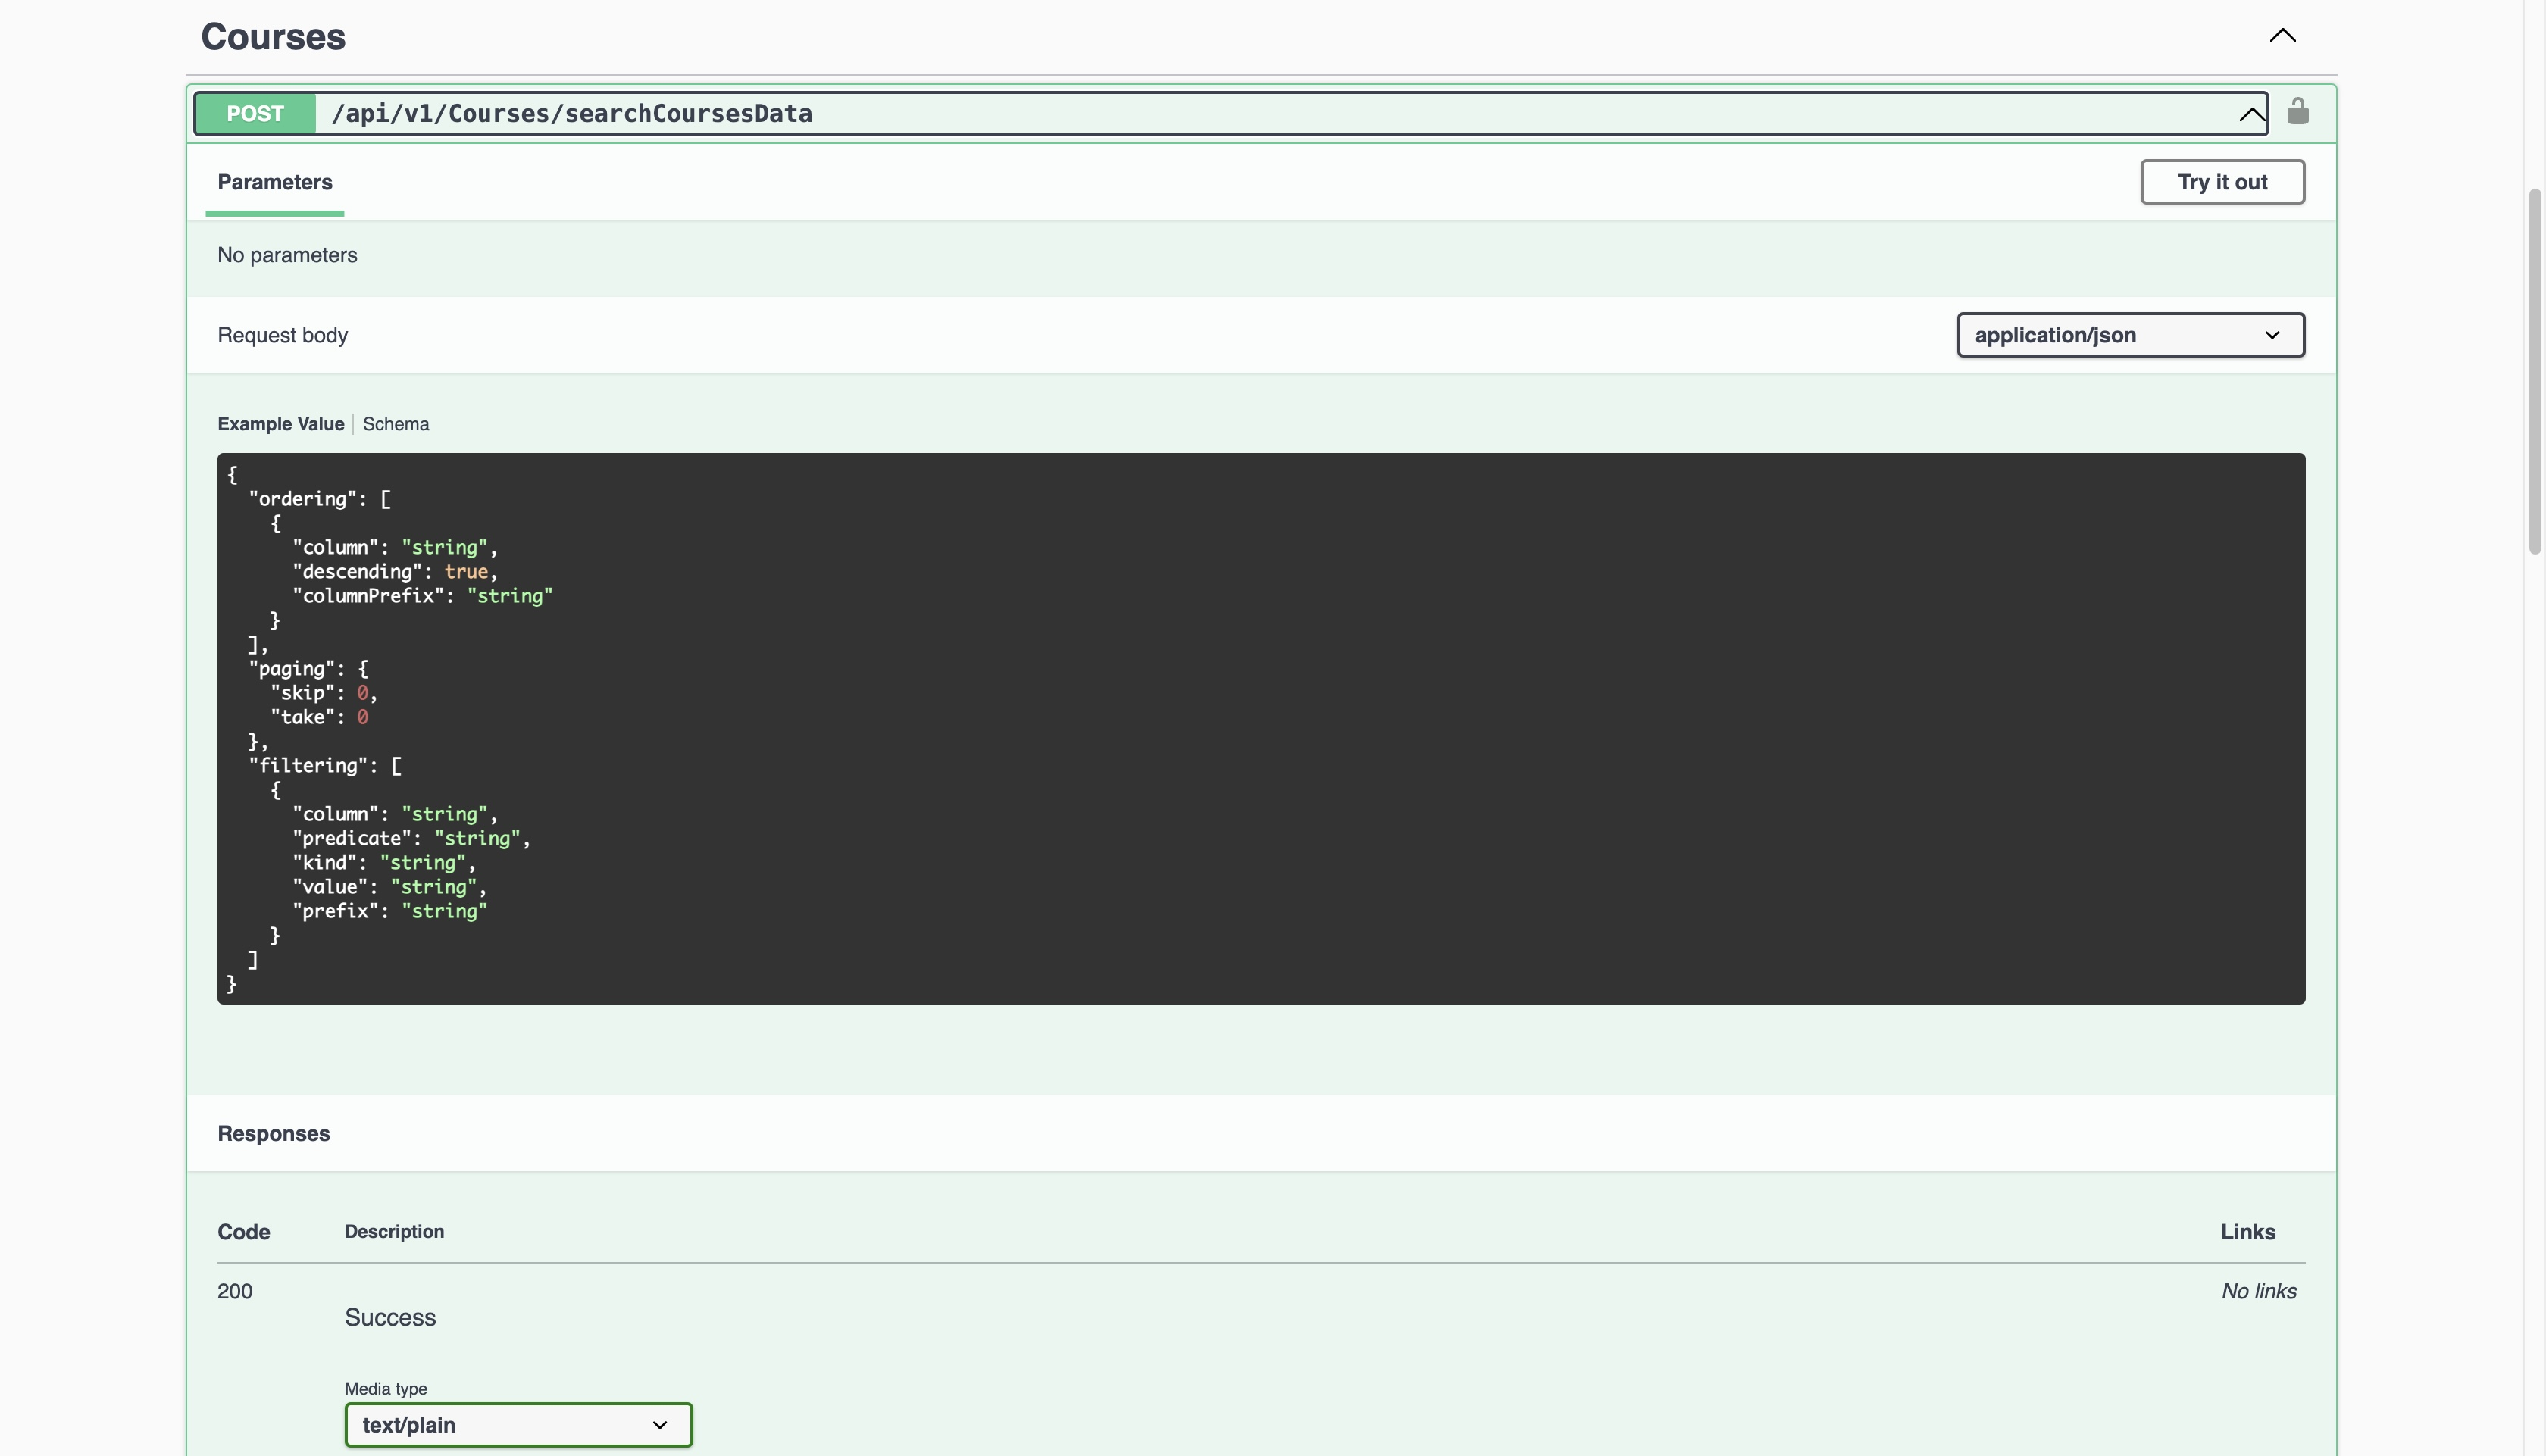
\includegraphics[width=1\textwidth]{Images/swagger courses.jpg}
\caption{\label{fig:swagger courses}Esempio di esecuzione di una \acrshort{api} per \texttt{searchCoursesData}, il corpo della richiesta è in formato \acrshort{json}.}
\end{figure}

\begin{figure}[H]
\centering
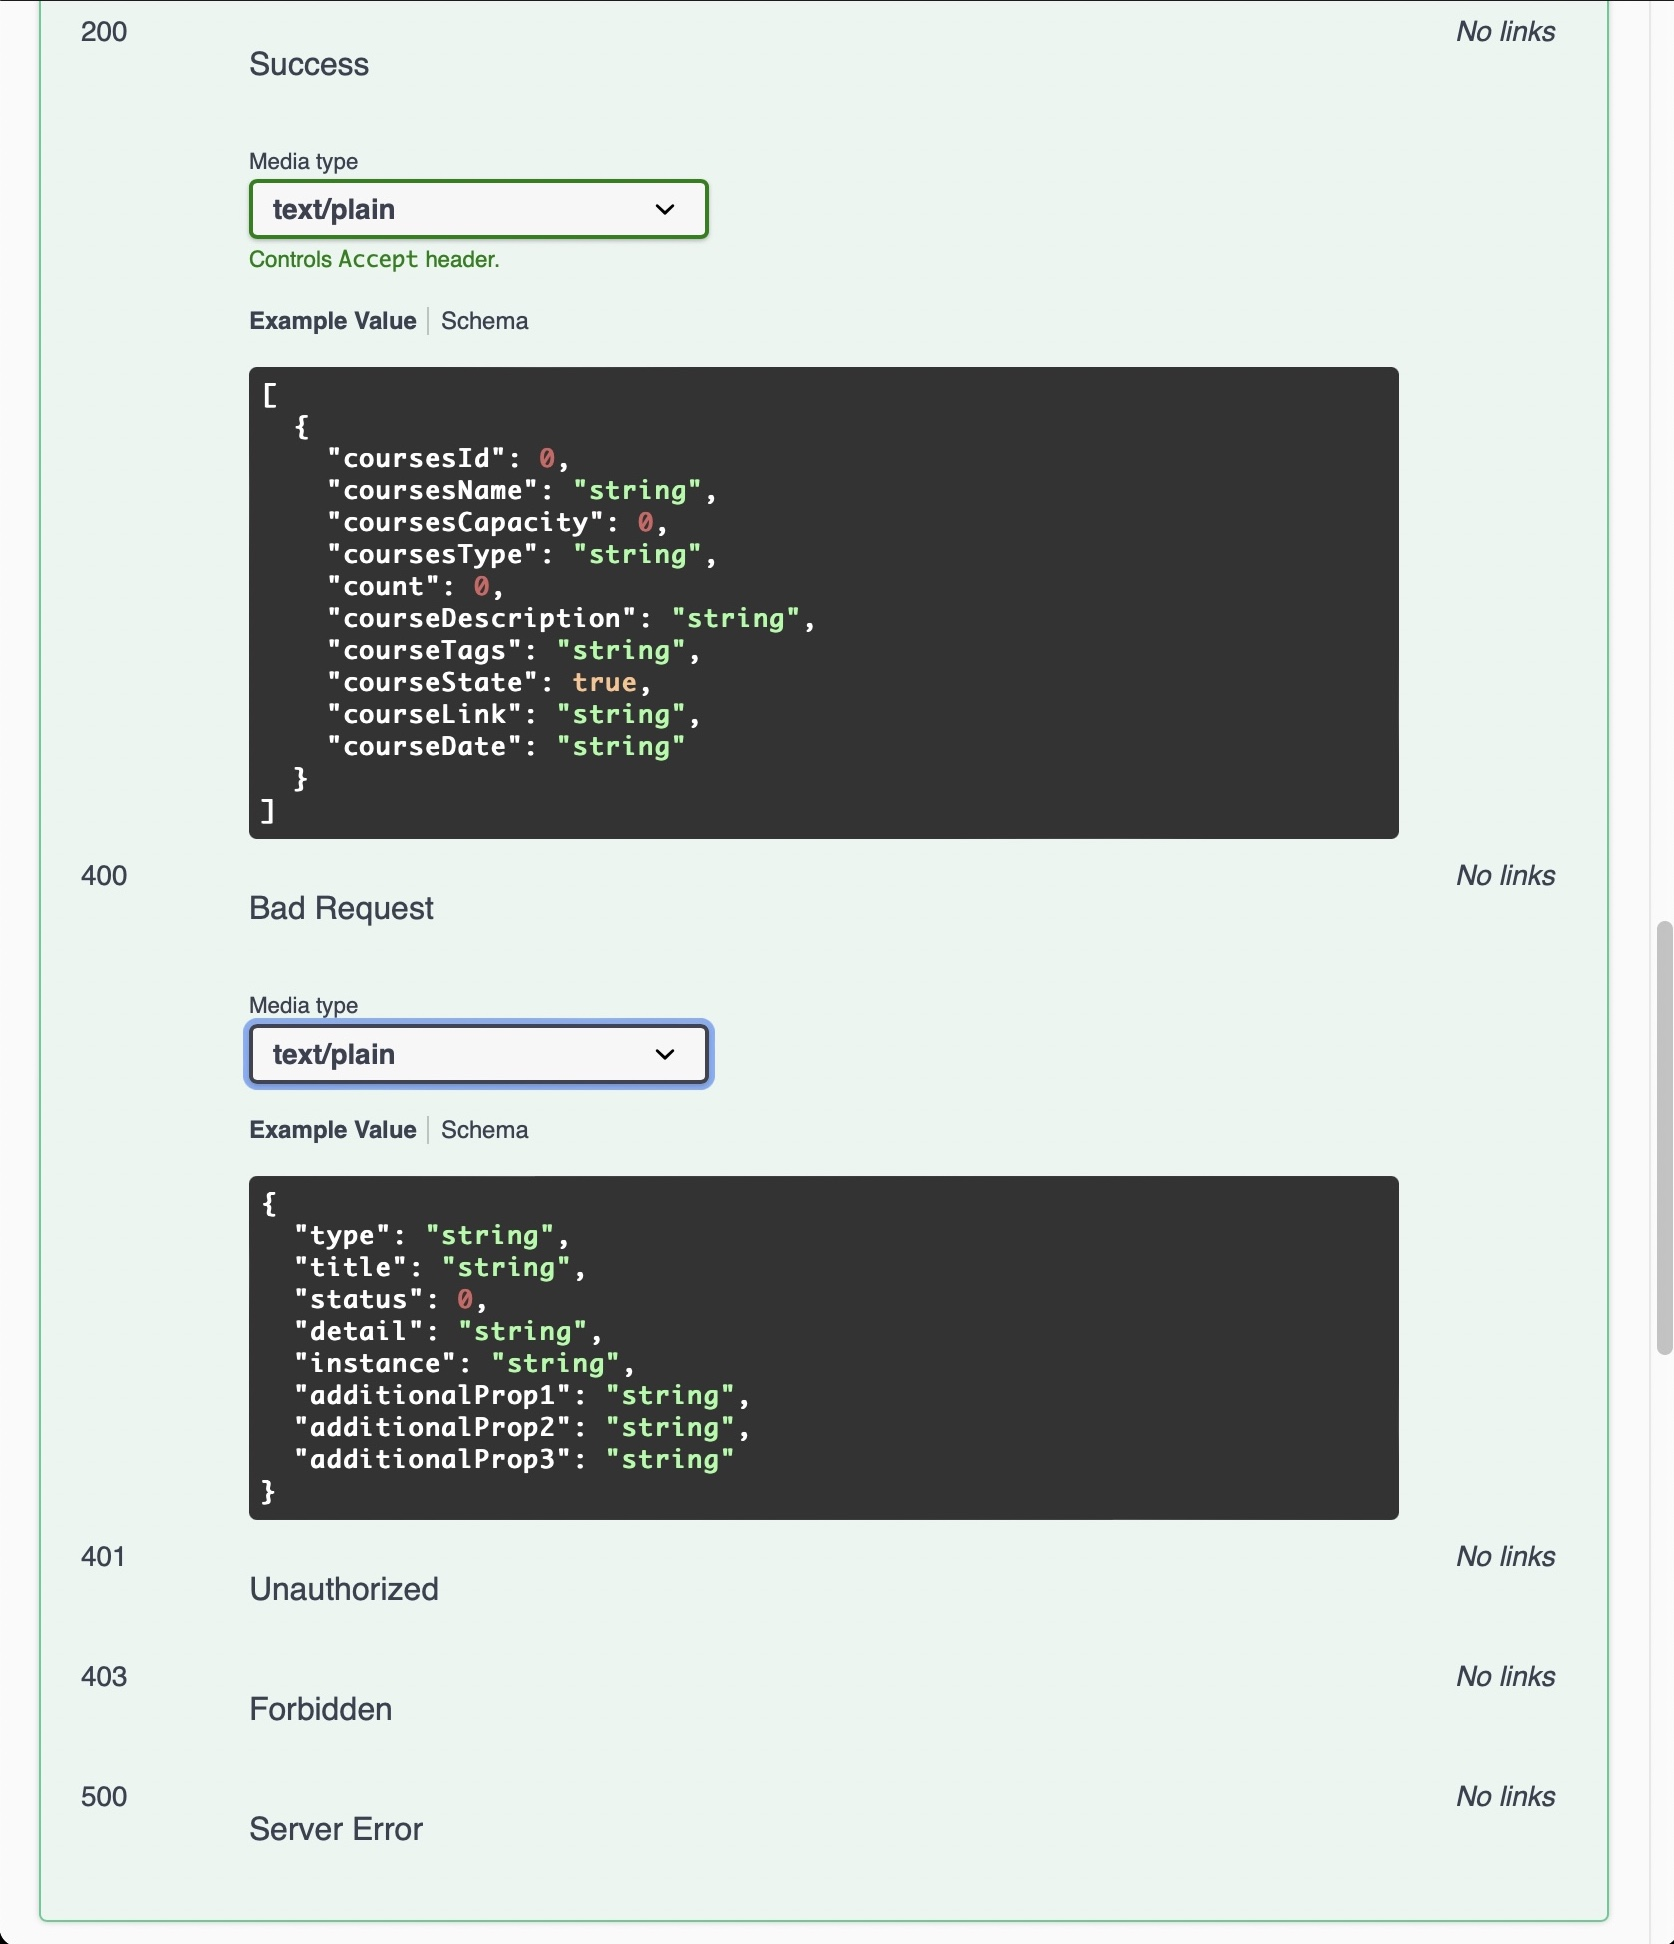
\includegraphics[width=1\textwidth]{Images/swagger success.jpg}
\caption{\label{fig:swagger success}Alcuni esempi di risultati di esecuzione di \acrshort{api} tramite Swagger, in ordine \texttt{200, Successo}, \texttt{400, `Cattiva richiesta'}, \texttt{401, `Non autorizzato'}, \texttt{403, `Vietato'} e \texttt{500, `Errore interno del server'}.}
\end{figure}


% front-end %%%%%%%%%%%%%%%%%%%%%%%%%%%%%%%%%%%%%%%%%%%%%%%%%%%%%%%%%%%%%%%%%%%%%%%%%%%%%%%
\section{Front-end}\label{sec:front-end}
Questa sezione descrive come ho usato \gls{angular} per lo sviluppo del front-end del prototipo.
Innanzitutto è stato necessario installare \acrfull{npm} e \acrfull{nvm}, i gestori di pacchetti rispettivamente per Angular e Node.js. In figura \ref{fig:installing nvm} si può vedere il listato del codice necessario per installarli, da riga di comando:
\begin{figure}[H]
\centering
\begin{lstlisting}[language=bash]
curl -o- https://raw.githubusercontent.com/nvm-sh/nvm/v0.39.0/   install.sh | bash
\end{lstlisting}
\caption{\label{fig:installing nvm}Comando per il terminale per scaricare e installare \acrshort{nvm}.}
\end{figure}
Successivamente, sempre da riga di comando, ho impostato la versione di \acrshort{nvm} necessaria per questo progetto, la numero 16, e poi ho installato le dipendenze necessarie, tramite il comando \texttt{npm install} \cite{nmpInstall}.

A questo punto, ho compilato e avviato il front-end tramite i comandi appositi \texttt{ng build} e \texttt{ng serve} in modo da poter accedere all'interfaccia grafica del prototipo, semplicemente accedendo ad un \acrshort{url} su un qualsiasi browser. Nella figura \ref{fig:ng serve} è mostrato l'output di un esempio di esecuzione del comando \texttt{ng serve} sul terminale.
\begin{figure}{}
\centering
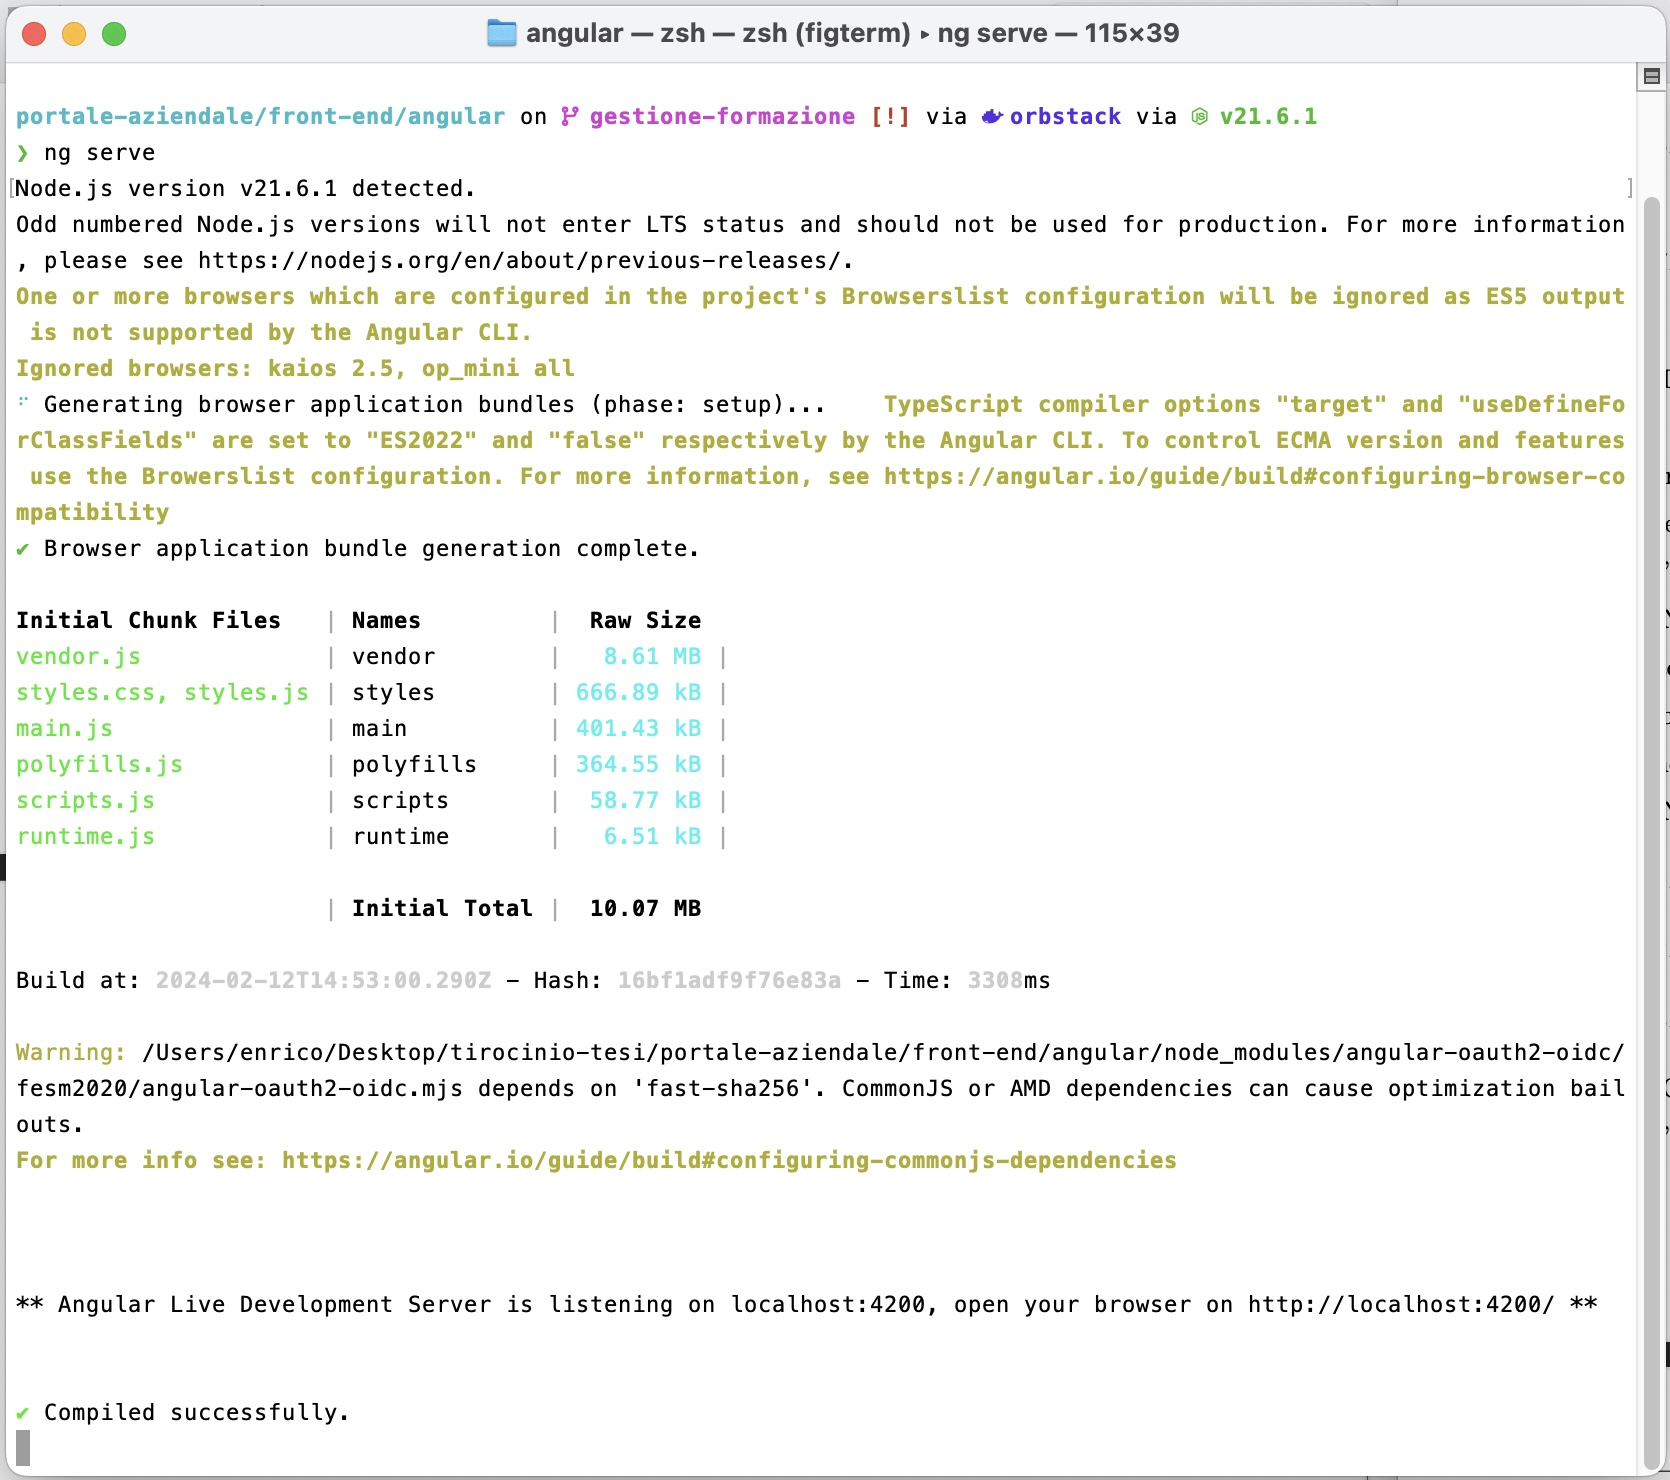
\includegraphics[width=.8\textwidth]{Images/ng serve.jpg}
\caption{\label{fig:ng serve}Screenshot di un terminale dopo aver eseguito \texttt{ng serve}.}
\end{figure}

Per la parte di sviluppo in \gls{angular}, ho utilizzato la sua \acrshort{cli}, che mi ha permesso di creare nuovi componenti, direttamente da terminale, con un solo comando. Per installarla è bastato eseguire \texttt{npm install -g @angular/cli} da riga di comando.
Se un nuovo componente viene creato senza errori, verrà creata una nuova cartella, chiamata con il nome del componente, all'interno del percorso \texttt{src/app/components}.
La cartella contiene fin dall'inizio tutti i file necessari per far funzionare il nuovo componente, come si può vedere in figura \ref{fig:education}.
\begin{figure}[H]
\centering
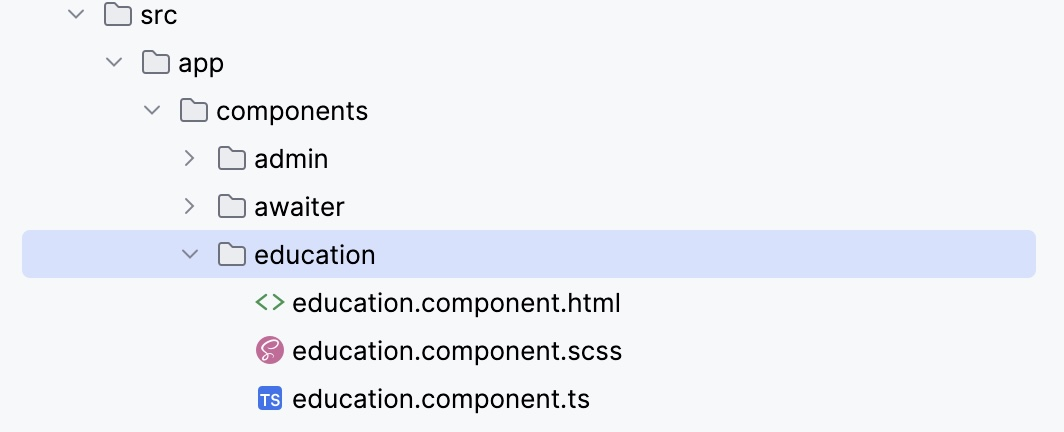
\includegraphics[width=1\textwidth]{Images/education.jpg}
\caption{\label{fig:education}Struttura della cartella del componente \texttt{education}, creata tramite la \acrshort{cli} di Angular.}
\end{figure}

Una volti creati i componenti, ho sviluppato il file \texttt{app-routing.module.ts}, che contiene la route guard di \gls{angular}. 
\begin{figure}[H]
\centering
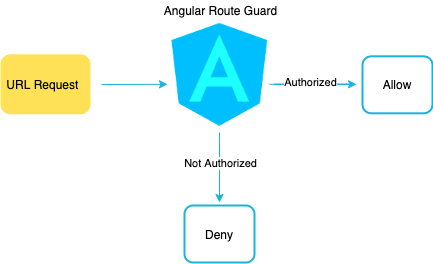
\includegraphics[width=.8\textwidth]{Images/routeguard.png}
\caption{\label{fig:routeguard}Schema di instradamento di \gls{angular}.}
\end{figure}
Una \texttt{route guard} in Angular è un meccanismo utilizzato per proteggere l'instradamento dell’applicazione e limitare l’accesso alle pagine in base alle autorizzazioni dell’utente. Le guardie consentono di gestire la navigazione dell’utente in modo sicuro, garantendo l’accesso alle pagine riservate solo agli utenti autorizzati (figura \ref{fig:routeguard}).
Una \texttt{route guard} è una classe \acrlong{ts} che implementa l’interfaccia \texttt{canActivate}, i cui metodi vengono eseguiti quando un utente tenta di accedere a una determinata rotta dell’applicazione.
Il metodo \texttt{canActivate}, ad esempio, viene eseguito quando un utente tenta di accedere a una route specifica. La \texttt{route guard} può quindi verificare se l’utente ha l’autorizzazione per accedere alla route e restituire un valore booleano che indica se l’accesso deve essere consentito o meno. Se la \texttt{route guard} restituisce \texttt{true}, l’utente può accedere, se invece restituisce \texttt{false}, l’utente viene reindirizzato a una pagina di errore o alla pagina di login. In figura \ref{fig:route guard} si può vedere il listato di un frammento di codice di una \texttt{route guard} sviluppata per questo progetto di tirocinio.
\begin{figure}[H]
\centering
\begin{lstlisting}[language=TypeScript]
export class AdminUserGuard implements canActivate {
    constructor(private oauthService: CustomOAuthService) {}

    async canActivate(
        route: ActivatedRouteSnapshot,
        state: RouterStateSnapshot
    ): Promise<boolean | UrlTree> {
        const isAdminUser = await this.oauthService.isAdminUser();
        if (!isAdminUser)
            console.error("You should be 'admin-user' to activate this route!");
        return isAdminUser;
    }
}
\end{lstlisting}
\caption{\label{fig:route guard}Metodo \texttt{canActivate} del file \texttt{admin-user.guard.ts}.}
\end{figure}
Una volta sviluppato il codice in figura \ref{fig:route guard} è stato necessario implementare il codice relativo al file \texttt{app-routing.module.ts} e l'instradamento dell'utente è completato. Il risultato è mostrato nelle seguenti figure.

\begin{figure}[!htb]
    \centering
    \begin{minipage}{.5\textwidth}
        \centering
        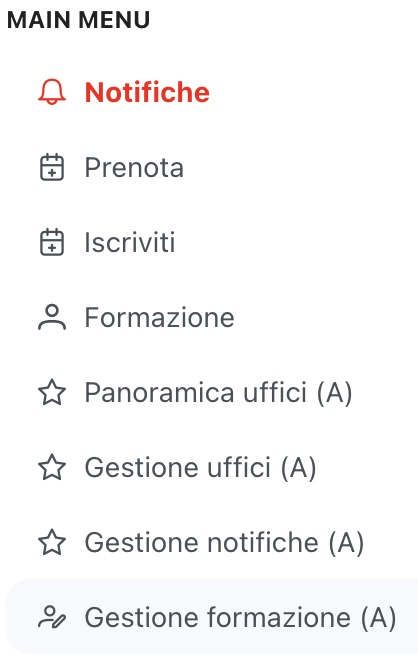
\includegraphics[width=.6\textwidth]{Images/admin.jpg}
        \centering
        \caption{\label{fig:admin}Vista dell'admin.}
    \end{minipage}%
    \begin{minipage}{0.5\textwidth}
        \centering
        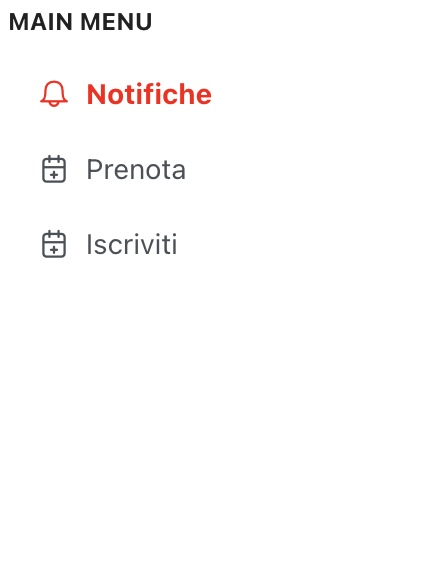
\includegraphics[width=.5\textwidth]{Images/base.jpg}
        \caption{\label{fig:base}Vista dell'utente base.}
    \end{minipage}
\end{figure}

Il codice di ogni componente è diviso nei tre file seguenti:
\begin{itemize}
  \item \texttt{`name'.component.html}, che si occupa di gestire la parte \acrshort{html} del componente, è quindi il template dello stesso;
  \item \texttt{`name'.component.ts}, che si occupa di gestire la parte TypeScript del componente;
  \item \texttt{`name'.component.css}, che in questo caso è vuoto, siccome il \acrshort{css} di ogni componente è stato gestito tramite il file \texttt{styles.css}.
\end{itemize}

In particolare, il file \acrshort{html} contiene lo `scheletro' del componente da visualizzare e alcuni tag speciali di \gls{angular} come, ad esempio, \texttt{ng-template pTemplate} nel listato \ref{fig:ptemplate}, che si occupa di uniformare i dati del back-end con le relative caselle di una tabella \acrshort{html}.

\begin{figure}[H]
\centering
\begin{lstlisting}[language=HTML]
 <ng-template pTemplate="body" let-coursesData>
    <tr class="p-selectable-row" [pRowToggler]="coursesData.coursesId">
        <td>
            <button type="button" pButton pRipple
                class="p-button-text p-button-rounded p-button-plain"
                [icon]="isRowExpanded(coursesData.coursesId) ? 'pi pi-chevron-down' : 'pi pi-chevron-right'"
                (click)="toggleRow(coursesData.coursesId)">
            </button>
        </td>
        <td>
            <span class="p-column-title">Nome corso</span>
            {{coursesData.coursesName}}
        </td>
    </tr>
</ng-template>
\end{lstlisting}
\caption{\label{fig:ptemplate}Frammento di codice \acrshort{html} del file \texttt{education.component.html}.}
\end{figure}

Per la parte \acrlong{ts} del componente, invece, è stato necessario considerare sia il livello di presentazione, che il livello di database, in modo da gestire e presentare le informazioni correttamente.
\begin{figure}[H]
\centering
\begin{lstlisting}[language=TypeScript]
addEducation(){
this.coursesData$.subscribe((data) => {
    if(data) {
        data.forEach((course) => {
            console.log(course);
    });}
});
\end{lstlisting}
\caption{\label{fig:education.ts}Metodo \texttt{addEducation()} del file \texttt{education.component.ts}.}
\end{figure}
Come mostrato in figura \ref{fig:education.ts}, il codice si occupa di aggiungere le informazioni trovate dal database (salvate in \texttt{coursesData\$()}) al front-end, in modo da essere visualizzate dall'utente.

\begin{figure}[H]
\centering
\begin{lstlisting}[language=CSS]
$gutter: 1rem; //for primeflex grid system
@import "assets/layout.scss";
@import "../node_modules/primeng/resources/primeng.min.css";
@import "../node_modules/primeflex/primeflex.scss";
@import "../node_modules/primeicons/primeicons.css";
@import "assets/overrides/styles/theme.scss";  
\end{lstlisting}
\caption{\label{fig:styles}\acrshort{css} del file \texttt{styles.css}, per gestire il \acrshort{css} di tutti i componenti.}
\end{figure}

La figura \ref{fig:styles} mostra lo stile dei componenti. Ho deciso di usare un tema predefinito di \acrshort{primeng}, importato nel file \texttt{styles.css}, come si può vedere nella figura. Nonostante la leggera perdita di personalizzazione, la scelta di utilizzare un tema predefinito mi ha permesso di ridurre i tempi di sviluppo, in quanto è stato necessario solamente importare un tema già pronto e non scrivere codice \acrshort{css} partendo da zero, cosa spesso complicata.

Altri file degni di nota sono:
\begin{itemize}
  \item \texttt{courses.actions.ts}: contiene tutti gli \texttt{export} delle azioni relative ai corsi di formazione;
  \item \texttt{courses.effects.ts}: si occupa principalmente di mappare le informazioni in entrata o in uscita dal componente;
  \item \texttt{courses.reducer.ts}: contiene alcuni metodi ausiliari per il corretto funzionamento della logica di business, in particolare per filtrare o manipolare le informazioni dal o verso il back-end;
  \item \texttt{courses.state.ts}: contiene la struttura di base dello stato dei corsi di formazione;
  \item \texttt{courses.selectors.ts}: che contiene gli \texttt{export} necessari per il funzionamento di ogni metodo filtro o di stato dei corsi di formazione.
\end{itemize}

Inoltre, dopo aver completato i file citati sopra, ho aggiunto un componente \gls{angular} per visualizzare un calendario visibile a larghezza intera, come si può vedere nella figura \ref{fig:fullcalendar} della pagina dell'applicazione web. Così facendo, l'utente può visualizzare i corsi di formazione esistenti e scegliere il corso di formazione più adatto alle proprie esigenze.
\begin{figure}[H]
\centering
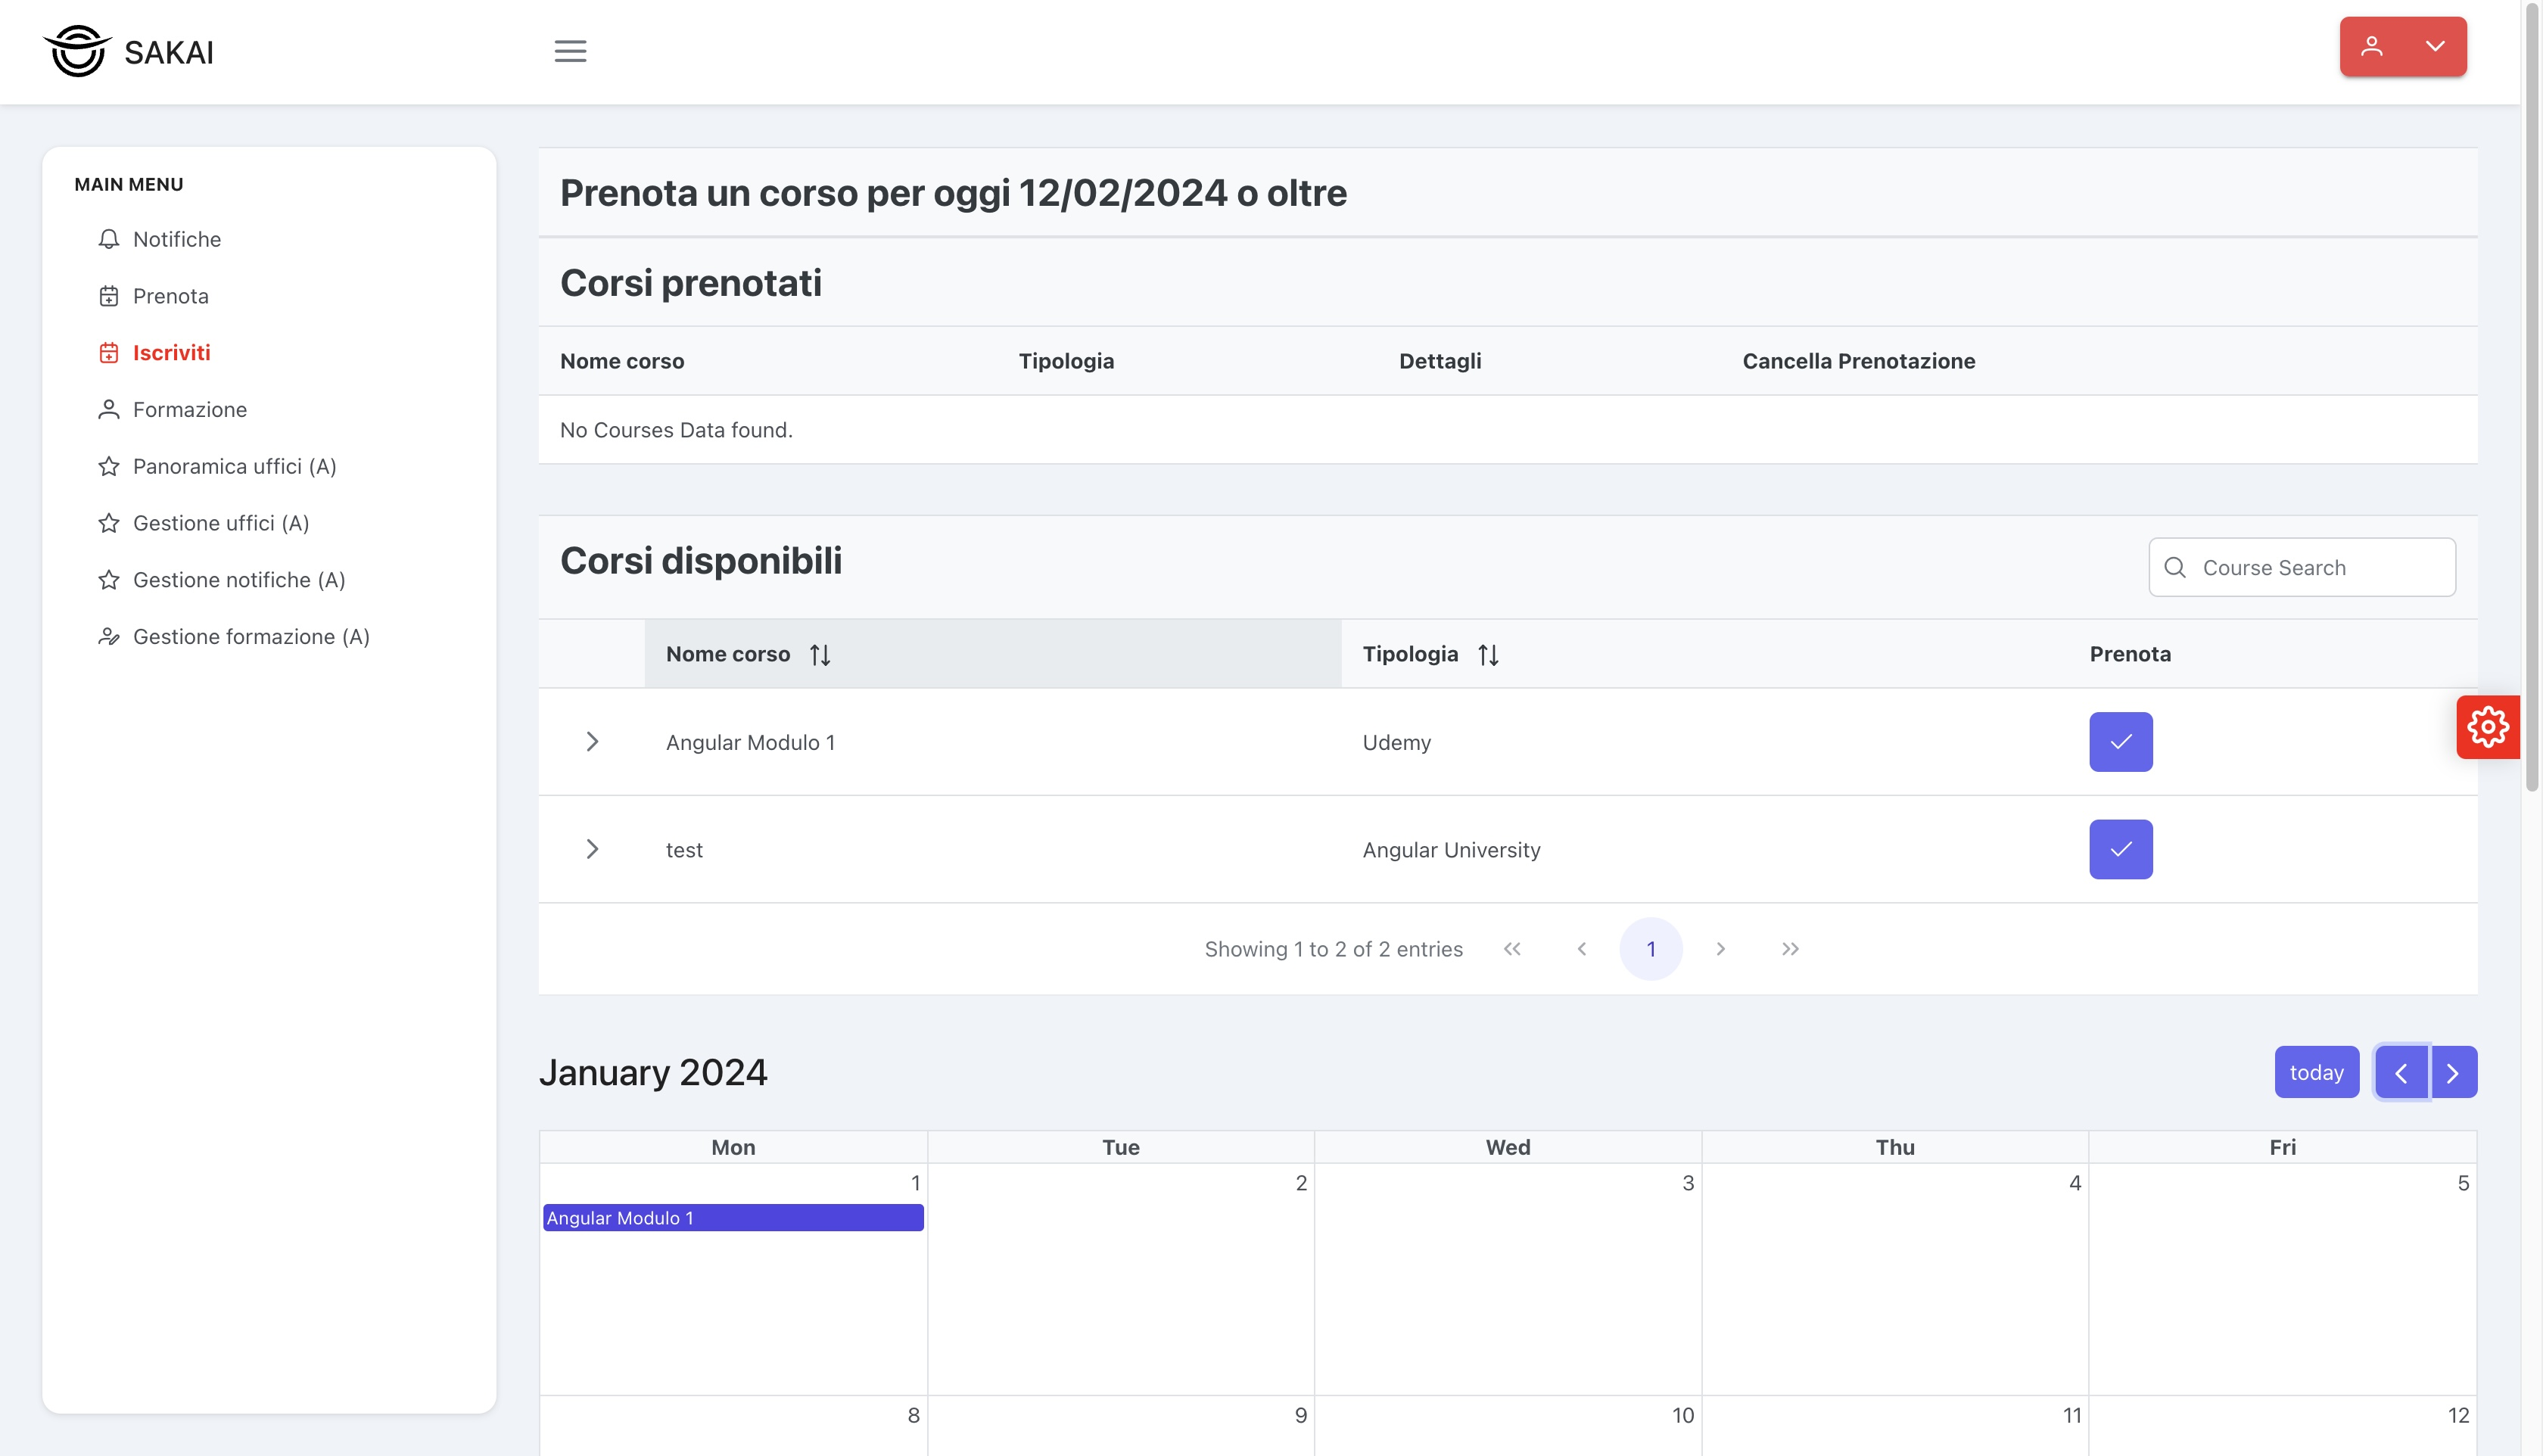
\includegraphics[width=1\textwidth]{Images/calendar cut.jpg}
\caption{\label{fig:calendar}Vista iniziale di una pagina web del prototipo, con il componente \texttt{fullcalendar}.}
\end{figure}

Dopo averlo installato, sempre tramite la \acrshort{cli} di \gls{angular} e aver configurato i file \texttt{app.module.ts} e \texttt{app.component.ts}, il calendario può funzionare correttamente \cite{fullcalendar}, come si può vedere in figura \ref{fig:fullcalendar}, semplicemente aggiungendo il tag \acrshort{html} apposito, mostrato nella figura \ref{fig:fullcalendar.html}:
\begin{figure}[H]
\centering
\begin{lstlisting}[language=HTML]
<full-calendar [options]="calendarOptions"></full-calendar>
\end{lstlisting}
\caption{\label{fig:fullcalendar.html}Tag \acrshort{html} del file \texttt{education.component.html}.}
\end{figure}

\begin{figure}[H]
\centering
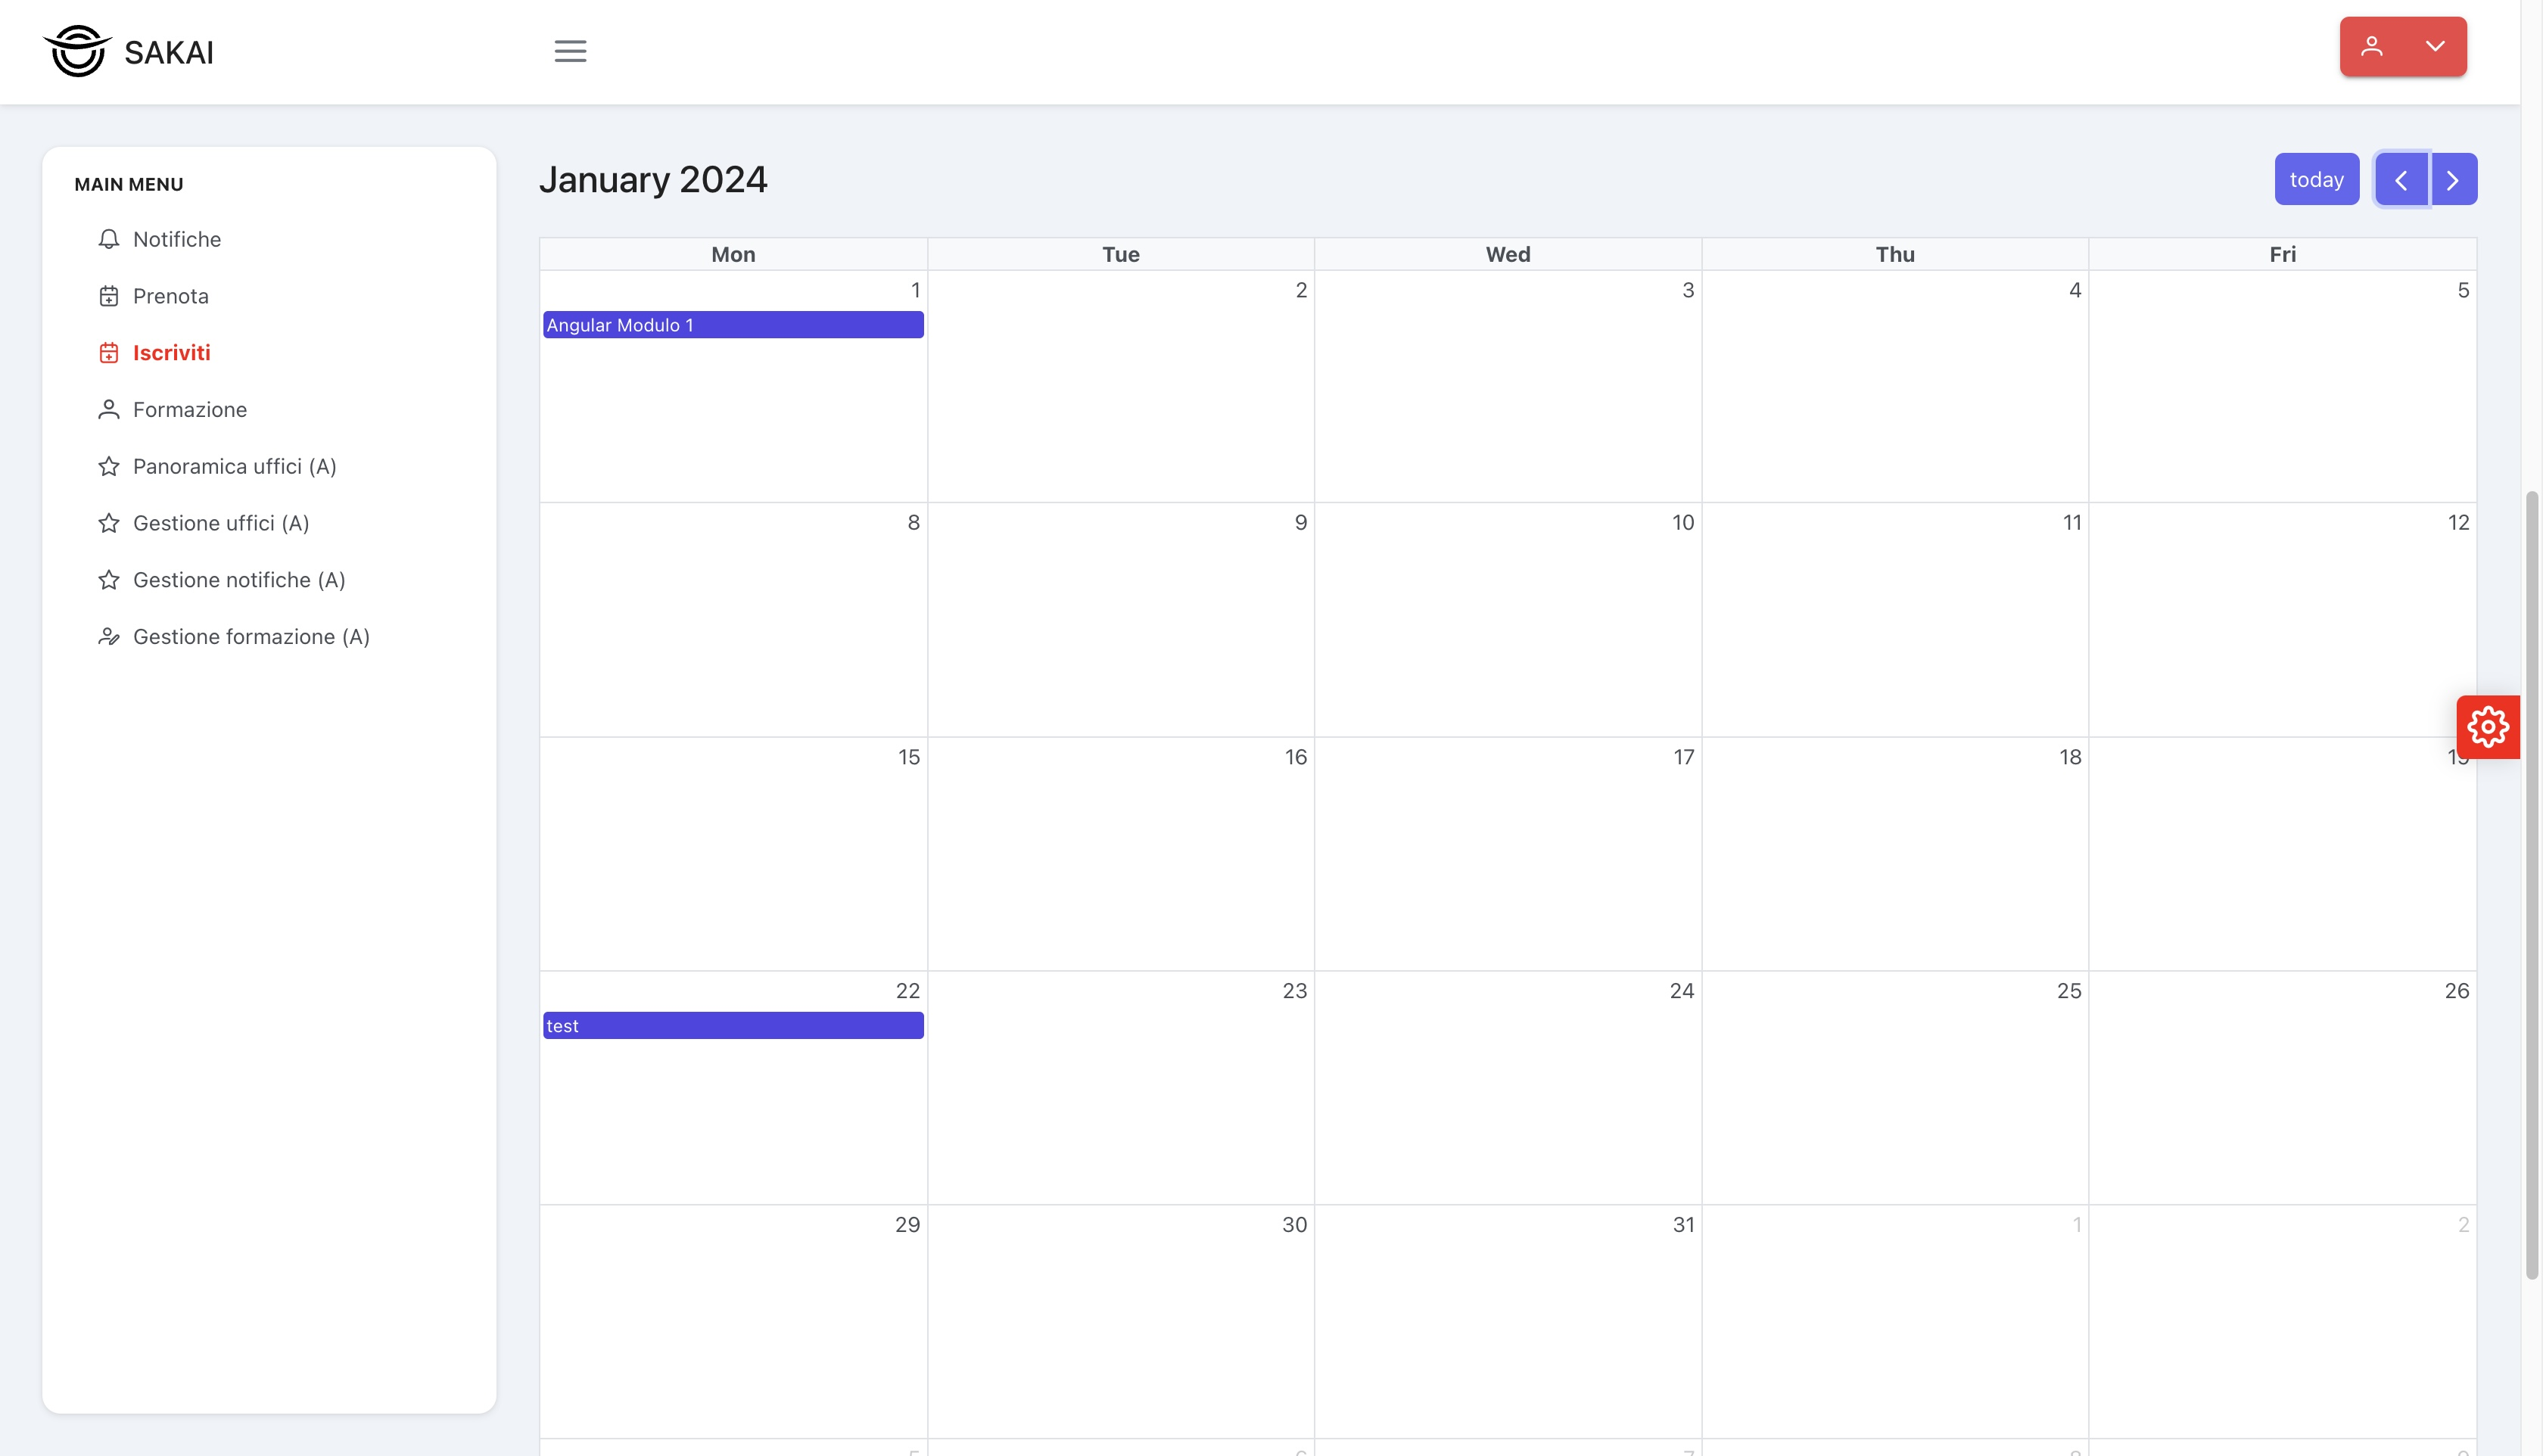
\includegraphics[width=1\textwidth]{Images/fullcalendar.jpg}
\caption{\label{fig:fullcalendar}Componente \texttt{fullcalendar}.}
\end{figure}

In figura \ref{fig:fullcalendar.ts} si può vedere il listato del codice \acrlong{ts}, per gestire la logica di business del componente \texttt{fullcalendarComponent}.

\begin{figure}[H]
\centering
\begin{lstlisting}[language=TypeScript]
ngOnInit(): void {
  this.coursesData$ = this.store.select(selectCoursesData).pipe(startWith( this.route .snapshot.data.CoursesData));
  this.coursesData$.pipe(
      filter(data => !!data)
  ).subscribe((data) => {
      this.totalRecords$ = this.coursesData$.pipe(map((x) => (x ? (x[0] ? x[0].count : 0) : 0)));
      let tmp = [];
      data.forEach((course) => {
          let day:string = course.coursesDate[0] + course.coursesDate[1];
          let month:string = course.coursesDate[3] + course.coursesDate[4];
          let year:string = course.coursesDate[6] + course.coursesDate[7] + course.coursesDate[8] + course.coursesDate[9];
          tmp.push({ title: course.coursesName, date: year + '-' + month + '-' + day }); // yyy-mm-dd
          console.log(tmp);
      });
      this.calendarOptions = {
          ...this.calendarOptions,
          events: tmp
      };
  })
}
\end{lstlisting}
\caption{\label{fig:fullcalendar.ts}\acrlong{ts} del file \texttt{education.component.ts}, necessario per il funzionamento della logica di business del calendario.}
\end{figure}

Lo sviluppo degli altri metodi e componenti è coerente agli esempi mostrati in precedenza e non verrà descritto in questo documento.
Infine, nella fase finale del tirocinio, ho aggiunto un componente per la gestione delle iscrizioni da parte degli utenti base. 
Anche in questo caso il codice è analogo ai file discussi in precedenza e non verrà descritto.


\subsection{PrimeNG}\label{subsec:primeng}
% Una veloce digressione su PrimeNG e su come l'ho usato e perchè \dots
Grazie a \acrshort{primeng}, ho potuto implementare un'interfaccia grafica funzionale e minimale.
Innanzitutto, è stato necessario installare i giusti pacchetti e le giuste dipendenze. Successivamente, la scelta dei componenti utilizzati e descritti in precedenza, è stata fatta in base alle esigenze del progetto e alle funzionalità offerte da \acrshort{primeng}.
In particolare, i componenti usati sono:
\begin{itemize}
  \item \texttt{p-table}, per la visualizzazione dei corsi di formazione;
  \item \texttt{p-sortableColumn} e \texttt{p-sortIcon}, per l'ordinamento dei dati della tabella;
  \item \texttt{p-inputText}, \texttt{p-dropdown}, \texttt{p-calendar}, per la gestione dei campi di input e delle date (figura \ref{fig:dropdown});
  \item \texttt{p-button}, per la gestione dei pulsanti di modifica e cancellazione;
  \item \texttt{p-fullCalendar}, per la visualizzazione dei corsi di formazione esistenti in un calendario;
  \item \texttt{ngtemplate}, per la gestione dei template personalizzati.
\end{itemize}
\begin{figure}[H]
\centering
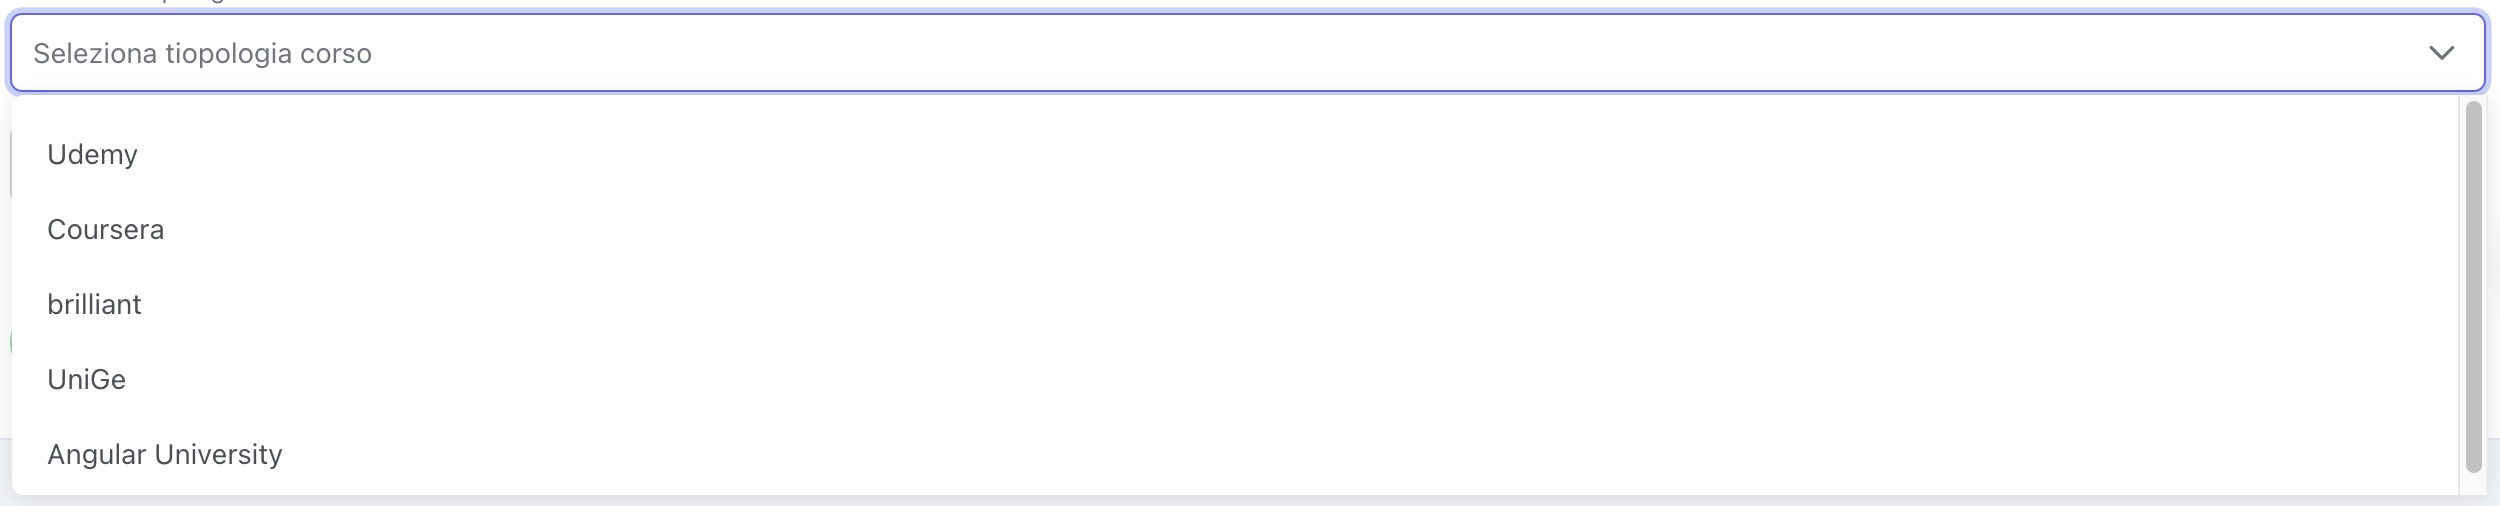
\includegraphics[width=1\textwidth]{Images/dropdown.jpg}
\caption{\label{fig:dropdown}Menù a tendina per la selezione della tipologia di un corso.}
\end{figure}


\subsection{Servizi Angular}\label{subsec:servizi-angular}
% Una veloce digressione sui servizi Angular e come sono stati usati \dots
I servizi \gls{angular} sono tra le funzionalità più potenti e flessibili del \gls{framework}, in quanto permettono di creare e gestire la logica di business in modo efficiente e modulare \cite{angserv}. Durante questo tirocinio, sono stati usati al fine di gestire la comunicazione tra il livello di presentazione e il livello della logica di business. Inoltre, sono stati scelti per la loro capacità di essere iniettati in qualsiasi componente.
Di seguito (figura \ref{fig:angular service} e \ref{fig:angular service 2}), si possono vedere due esempi di come è stato usato un servizio \gls{angular} per la gestione dei corsi di formazione:
\begin{figure}[H]
\centering
\begin{lstlisting}[language=TypeScript]
  @Injectable({ providedIn: "root" })
\end{lstlisting}
\caption{\label{fig:angular service}\acrlong{ts} del file \texttt{course.resolver.ts}, contenente l'implementazione di un servizio \gls{angular}.}
\end{figure}

\begin{figure}[H]
\centering
\begin{lstlisting}[language=TypeScript]
  @Injectable({ providedIn: "any" })
\end{lstlisting}
\caption{\label{fig:angular service 2}\acrlong{ts} del file \texttt{admin-user-guard.ts}, contenente l'implementazione di un servizio \gls{angular}.}
\end{figure}

% `